% TEX program = xelatex
\documentclass{beamer}
% \usepackage[fontset=fandol]{ctex}
%\documentclass[aspectratio=169]{beamer} % 使用 16:9 宽屏比例
% \usepackage{ctex}
\usepackage{hyperref}
\usepackage[T1]{fontenc}

% other packages
\usepackage{latexsym,amsmath,xcolor,multicol,booktabs,calligra}
\usepackage{graphicx,pstricks,listings,stackengine}

\author{MOREANU Vlad, PATRASCU Cosmin}
\title{Single-Channel Speech Separation}
\subtitle{The influence of additive noise on blind source separation}
\institute{National University of Science and Technology POLITEHNICA Bucharest}
\date{08/04/2026}
\usepackage{CNU}

% defs
\def\cmd#1{\texttt{\color{red}\footnotesize $\backslash$#1}}
\def\env#1{\texttt{\color{blue}\footnotesize #1}}
\definecolor{deepblue}{rgb}{0,0,0.5}
\definecolor{deepred}{rgb}{0.6,0,0}
\definecolor{deepgreen}{rgb}{0,0.5,0}
\definecolor{halfgray}{gray}{0.55}

% \lstset{
%     basicstyle=\ttfamily\small,
%     keywordstyle=\bfseries\color{deepblue},
%     emphstyle=\ttfamily\color{deepred},    % Custom highlighting style
%     stringstyle=\color{deepgreen},
%     numbers=left,
%     numberstyle=\small\color{halfgray},
%     rulesepcolor=\color{red!20!green!20!blue!20},
%     frame=shadowbox,
% }

\begin{document}

\begin{frame}
    \titlepage
    \begin{figure}[htpb]
        \begin{center}
            % 
\includegraphics[width=0.4\linewidth]{pic/logo.png}
        \end{center}
    \end{figure}
\end{frame}

% \begin{frame}
%     \tableofcontents[sectionstyle=show,subsectionstyle=show/shaded/hide,subsubsectionstyle=show/shaded/hide]
% \end{frame}

\section{Task Description}

\begin{frame}{Task Description}
    \begin{itemize} % [<+-| alert@+>] 
        \item Analyse the performance of a separation model as the signal-to-noise ratio (SNR) decreases.
        \item Input: Mixture signal with noise of varying levels
        \item Measure the discrepancy between the estimated sources and the true sources
    \end{itemize}
\end{frame}

\section{Baseline model}
\begin{frame}{Baseline model}
    Trained for 150 epochs on the clean subset with checkpoints monitoring
    val\_loss.
    \begin{multicols}{2}
        \begin{itemize}
            \item $ N = 128 $
            \item $ L = 20 $
            \item $ B = 128 $
            \item $ H = 64 $
            \item $ P = 3 $
            \item $ X = 2 $
            \item $ R = 4 $
            \item $ C = 2 $
            \item $ \text{mask\_nonlinear} = \text{"sigmoid"} $
        \end{itemize}
        \columnbreak
        \begin{itemize}
            \item $ lr = 0.001 $
            \item $ \text{weight\_decay} = 0 $
        \end{itemize}
    \end{multicols}
\end{frame}

\section{The Noise} 
\begin{frame}{Choice of noise values}
    \begin{itemize}
        \item Additive White Gaussian Noise $\mathcal{N}(0, \sigma^2)$.
        \item Chosen sigma values:
        \begin{itemize}
            \item $\sigma = 0.005 \implies \text{SNR} \approx 19.89 \text{ dB}$
            \item $\sigma = 0.01 \implies \text{SNR} \approx 13.85 \text{ dB}$
            \item $\sigma = 0.02 \implies \text{SNR} \approx 7.83 \text{ dB}$
        \end{itemize}
    \end{itemize}
\end{frame}

\section{Training Strategy}
\begin{frame}{Training Strategy}
    \begin{itemize}
        \item 50 epochs with clean sources as targets
        and noisy mixtures as inputs
        \item Transfer learning from baseline
        \item Chosen $\sigma = 0.01$ as the other two result in noise that is
        either too inconsequential or too destructive. 
    \end{itemize}
\end{frame}

\section{Results}

\begin{frame}{Table of Results}
    \begin{table}
        \centering
        \resizebox{\textwidth}{!}{%
            \begin{tabular}{|l|c|c|c|}
                \hline
                \textbf{Model}
                &
                \textbf{$\sigma=0.005(SNR=19.89dB)$}
                &
                \textbf{$\sigma=0.01(SNR=13.85dB)$}
                &
                \textbf{$\sigma=0.02(SNR=7.83dB)$}
                \\
                \hline
                \textbf{Original model}
                &
                \textbf{-4.22}
                &
                \textbf{-3.62}
                &
                \textbf{-1.86}
                \\
                \hline
                \textbf{Trained on $\sigma_2$}
                &
                \textbf{-4.50}
                &
                \textbf{-4.21}
                &
                \textbf{-3.13}
                \\
                \hline
            \end{tabular}%
        }
        \caption{Results - SI-SNR-PIT on test set}
    \end{table}
\end{frame}

% \begin{frame}{Mixed Signal}
%     \begin{figure}
%         \centering
%         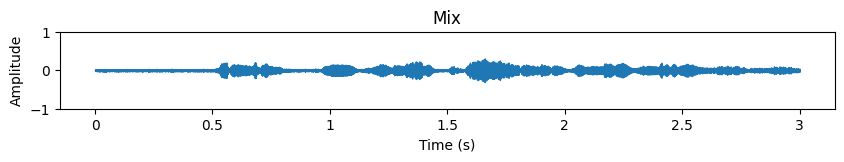
\includegraphics[width=1\linewidth]{pic/mixed.png}
%         \caption{Plot of Mixed Signals}
%     \end{figure}
% \end{frame}

\begin{frame}{First Source}
    \begin{figure}
        \centering
        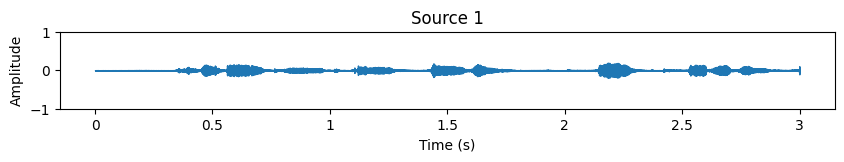
\includegraphics[width=1\linewidth]{pic/s1.png}
    \end{figure}

    \begin{figure}
        \centering
        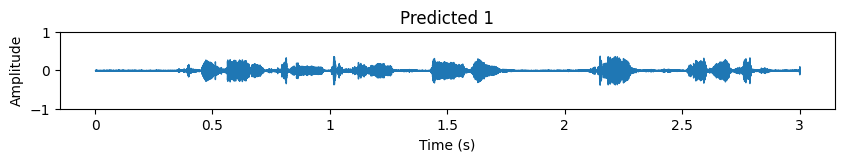
\includegraphics[width=1\linewidth]{pic/p1.png}
    \end{figure}
\end{frame}

\begin{frame}{Second Source}
    \begin{figure}
        \centering
        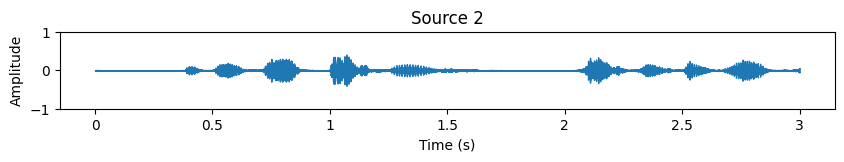
\includegraphics[width=1\linewidth]{pic/s2.png}
    \end{figure}

    \begin{figure}
        \centering
        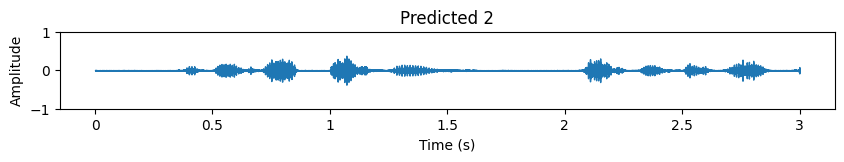
\includegraphics[width=1\linewidth]{pic/p2.png}
    \end{figure}
\end{frame}


% \section{section5}

% \begin{frame}{xxxxxx}
%     \bibliographystyle{plain}
%     \bibliography{ref} % refers to ref.bib
% \end{frame}

% \begin{frame}
%     \begin{center}
%         {\Huge\calligra Thanks!}
%     \end{center}
% \end{frame}

\end{document}